\section{Making Canonical Workflow Building Blocks interoperable across
workflow
languages}
\label{ch6:making-canonical-workflow-building-blocks-interoperable-across-workflow-languages}

We introduce the concept of \emph{Canonical Workflow Building Blocks}
(CWBB), a methodology of describing and wrapping computational tools, in
order for them to be utilised in a reproducible manner from multiple
workflow languages and execution platforms. The concept is implemented
and demonstrated with the BioExcel Building Blocks library (BioBB), a
collection of tool wrappers in the field of computational biomolecular
simulation. Interoperability across different workflow languages is
showcased through a protein Molecular Dynamics setup transversal
workflow, built using this library and run with 5 different Workflow
Manager Systems (WfMS). We argue such practice is a necessary
requirement for FAIR Computational Workflows and an element of Canonical
Workflow Frameworks for Research (CWFR) in order to improve widespread
adoption and reuse of computational methods across workflow language
barriers.

\subsection{Introduction}\label{ch6:introduction}

The need for \emph{reproducibility} of research software usage is well
established \cite{Stodden 2016,Leipzig 2021,ch6-3}, and adaptation of \emph{workflow management
systems} (\textbf{WfMS}) together with \emph{software packaging and
containers} \cite{ch6-4} have been proposed as key ingredients for making
research software usage \emph{FAIR} and reproducible \cite{Cohen-Boulakia 2017,Gruning 2018b,Lamprecht 2019}.
Recently it is also argued that computational workflows should also be
treated as FAIR Digital Objects \cite{De Smedt 2020} in their own right, with
identifier, metadata \cite{Leipzig 2021} and interoperability requirements \cite{Goble 2020}.

\footurl{https://bioexcel.eu/}{BioExcel}, a European Centre of Excellence
for Computational Biomolecular Research, has a particular focus on the
research domains molecular dynamics simulations and bioinformatics with
use of \emph{High Performance Computing} (\textbf{HPC}) to approach
Exascale performance, while also improving usability. The \emph{BioExcel
Building Blocks} (\textbf{BioBB}) \cite{ch6-10} have been created as portable
wrappers of open-source computational tools identified as useful for
BioExcel workflows, forming several \emph{families} of documented and
interoperable operations that can be called from multiple workflow
systems. This interoperability is shown with the BioBB demonstrator
workflows, along with multiple tutorials and notebooks.

We propose that these building blocks and their families can themselves
be considered \emph{composite Digital Objects}: collections of software
packages and their source code, guides and tutorials, as well as
workflow management system integrations and workflow examples. In
addition, the building blocks, as wrappers of upstream open source
tools, benefit from and refer to the tools' existing documentation,
support forums, academic publications and wider development context.

Given BioBB as a starting point, we define a generalized methodology of
\emph{Canonical Workflow Building Blocks} (\textbf{CWBB}), through the
definition of a set of requirements and recommendations for how to
formalize and develop a family of compatible computational tools as
Digital Objects. These building blocks let researchers instantiate a
Canonical Workflow in multiple workflow management systems, while also
benefiting from the FAIR aspects of the CWBB Digital Objects.

\subsection{Methods}\label{ch6:methods}

The \footurl{http://mmb.irbbarcelona.org/biobb/}{BioExcel Building Blocks}
library \cite{ch6-10}, created and implemented within the BioExcel CoE, is a
collection of portable wrappers of common biomolecular simulation tools.
The BioBB library is designed to i) increase the \emph{interoperability}
between the tools wrapped; ii) \emph{ease the implementation} of
biomolecular simulation workflows; and iii) increase the
\emph{reusability and reproducibility} of the generated workflows. To
achieve these main goals, the library was designed following the FAIR
principles for research software development best practices \cite{Lamprecht 2019}.

The result is a collection of building block modules, divided in sets of
tool wrappers focused on similar functionalities (e.g.~Molecular
Dynamics, Virtual Screening). Each of the modules is built from a
combination of (i) software packaging
(\footurl{https://pypi.org/project/biobb/}{Pip},
\footurl{https://bioconda.github.io/search.html?q=biobb}{BioConda},
\footurl{https://biocontainers.pro/}{BioContainers}), (ii) documentation
(\footurl{https://biobb.readthedocs.io/}{ReadTheDocs}), (iii) interactive
tutorials
(\footurl{http://mmb.irbbarcelona.org/biobb/workflows/tutorials/md_setup}{Jupyter
Notebooks},
\footurl{https://bioexcel-binder.tsi.ebi.ac.uk/v2/gh/bioexcel/biobb_wf_md_setup/master?filepath=biobb_wf_md_setup\%2Fnotebooks\%2Fbiobb_MDsetup_tutorial.ipynb}{Binder}),
(iv) registry \& findability (\footurl{https://bio.tools/biobb}{bio.tools},
\footurl{https://bioschemas.org/profiles/ComputationalTool/0.5-DRAFT/}{BioSchemas},
\footurl{https://workflowhub.eu/programmes/2}{WorkflowHub}), (v) WfMS
integration stubs
(\footurl{https://github.com/bioexcel/biobb_adapters/tree/v0.1.4/biobb_adapters/cwl}{CWL},
\footurl{https://toolshed.g2.bx.psu.edu/repository?repository_id=e23296b413014cfc}{Galaxy},
\footurl{https://github.com/bioexcel/biobb_adapters/tree/v0.1.4/biobb_adapters/pycompss}{PyCOMPSs}),
(vi) source Code (\footurl{https://github.com/bioexcel/biobb}{GitHub}) and
(vii) REST APIs
(\footurl{https://mmb.irbbarcelona.org/biobb-api/rest}{OpenAPI},
\footurl{https://mmb.irbbarcelona.org/biobb-api/rest/swagger.json}{Swagger}).
Notably all building blocks follow the same pattern of installation,
configuration and interaction.

Since the publication of the library, several
\footurl{https://mmb.irbbarcelona.org/biobb/documentation/source}{new
building block modules} (Chemistry, Machine Learning, AMBER MD, Virtual
Screening, etc.) have been added, and the set of operations for the
existing BioBB families have been expanded. While we previously provided
curated adapters (Figure \vref{ch6:figure1}) for running BioBB in workflow systems using
Common Workflow Language (CWL) and PyCOMPSs, along with Galaxy Toolshed
bindings, we have now started auto-generating these bindings, along with
command line wrappers and REST web service APIs, using annotations
within BioBB's Python docstrings as source. These annotations include
sufficient information for a WfMS to launch a particular building block:
\emph{input} and \emph{output} parameters (including
\emph{mandatory/optional} flags), compatible \emph{formats} (including
from EDAM ontology \cite{ch6-11}), \emph{example} files (essential for
testing purposes), default values and \emph{dependencies}. This ensures
human-readable documentation, FAIR metadata and programmatic
accessibility can be generated consistently and comparably.

\begin{figure}%[t]
  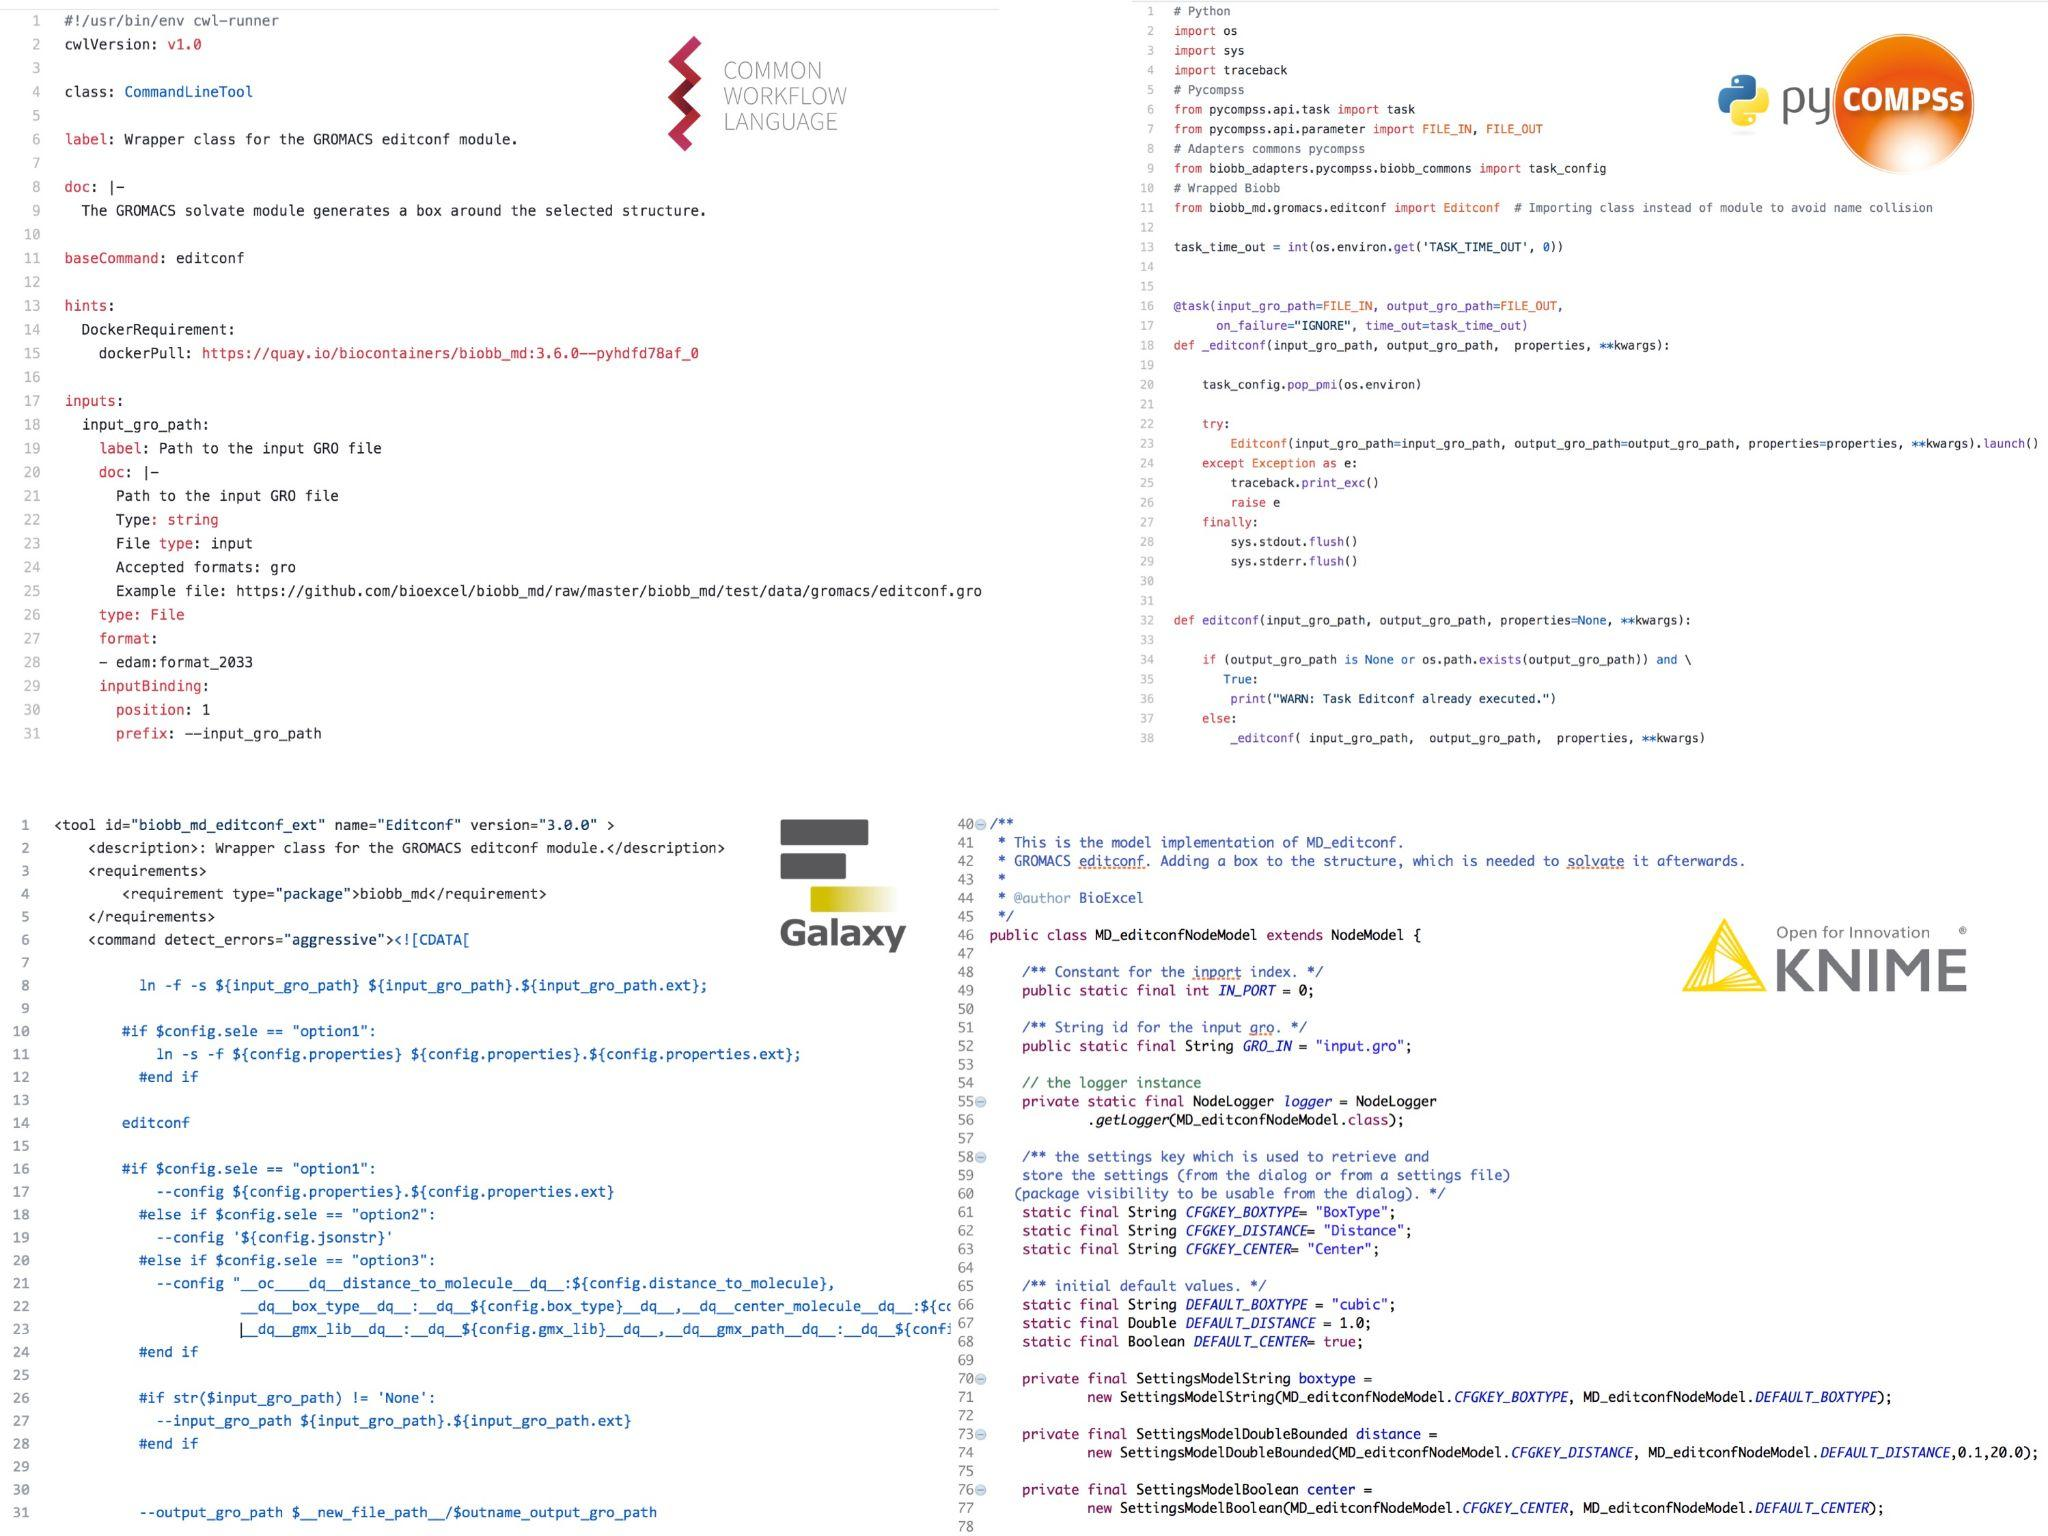
\includegraphics[width=\textwidth]{figures/ch06/figure1.jpg}
	\caption[Code snippets for the BioBB
  WfMS bindings]{\textbf{Code snippets for the BioBB
  WfMS bindings}: CWL, PyCOMPSs, Galaxy and KNIME.}
  \label{ch6:figure1}
\end{figure}

The library is showcased through a collection of
\footurl{http://mmb.irbbarcelona.org/biobb/workflows}{demonstration
workflows} \cite{ch6-12}. Here, each workflow introduces individual building
blocks as needed to explain a particular scientific computational
method. We primarily expose the workflows as Jupyter Notebooks \cite{Kluyver 2016},
which has been highlighted as a valuable tool for reproducible
scientific workflows \cite{ch6-14}. This offers a graphical interactive
interface, including documentation (integrated markdown) related to the
workflow and the building blocks used, but also to the biomolecular
simulation methods used in the pipeline. Moreover, as we have
demonstrated with our own
\footurl{https://hub-bioexcel-binder.tsi.ebi.ac.uk/}{Binder} \cite{ch6-15}
hosting, these workflows are reproducible across platforms, assisted by
BioConda \cite{Gruning 2018a} packaging of the building blocks and their software
dependencies.

This assembly of available demonstration workflows have been
successfully used in the BioExcel CoE for dissemination with a range of
\footurl{https://mmb.irbbarcelona.org/biobb/about/training}{training
events} (e.g.~BioExcel Summer \& Winter School, webinars and virtual
training). In training we particularly utilised the Binder
infrastructure of the BioExcel Cloud portal \cite{ch6-17} to give users a
web-based first experience of the building blocks before they try them
in other workflow systems.

We can observe that workflow building blocks such as BioBB are
necessarily composed of a comprehensive list of digital objects,
encompassing source code, packaging, containerization, documentation,
attributions, citations, registry entries, WfMS integrations and REST
APIs.

We propose to consider building blocks as \emph{composite digital
objects} in their own right: gathering the above software components
along with their metadata, identifiers and operations then forms a
\emph{Canonical Workflow Building Block} (\textbf{CWBB}). We suggest
this concept as a fundamental element of FAIR Digital Objects for
Computational Workflows: researchers use the building blocks
computationally as functional operations across WfMSs, while the FAIR
aspect of CWBB propagates information and resources that are essential
for reproducibility, reuse and understanding by anyone discovering the
workflow.

\subsubsection{Interoperability across different workflow
languages}\label{ch6:interoperability-across-different-workflow-languages}

The concept of Canonical Workflow Building Blocks is here showcased with
the BioBB library, by using a transversal workflow present in many
different computational biomolecular projects: a
\footurl{http://mmb.irbbarcelona.org/biobb/workflows/tutorials/md_setup}{Molecular
Dynamics (MD) protein setup}. This workflow prepares a protein structure
to be used as input for an MD simulation, going through a series of
steps where the protein is completed (adding hydrogen and missing
atoms), optionally introducing a residue mutation, then submerging the
protein in a virtual box of water molecules with a particular ionic
concentration, and finally energetically equilibrating the system (so
that solvent and ions are well accommodated around the protein at the
desired temperature).

This simulation process involves a non-negligible number of steps, using
a variety of biomolecular tools. The BioBB library was used to assemble
this workflow, interconnecting building blocks using Python functions
(Jupyter Notebook, Command Line Interface), auto-generated bindings
(Galaxy \cite{Afgan 2018}, CWL \cite{Crusoe 2022}, PyCOMPSs \cite{ch6-20}) or manually generated
bindings (KNIME \cite{ch6-21}). Corresponding workflows for the different
WfMS can be found in
\footurl{https://workflowhub.eu/collections/3}{WorkflowHub} \cite{ch6-22,ch6-23,ch6-24,ch6-25,ch6-26}
and graphical extracts can be seen in Figure \vref{ch6:figure2}.

This example demonstrates how the same canonical building blocks can be
used in different WfMS. Wrappers and tools executed behind the workflows
are exactly the same, but the workflows are built using different WfMS,
some of them in a graphical way (drag \& drop, Galaxy, KNIME), some in a
command line way (Jupyter Notebook, PyCOMPSs, CWL); workflows can be
focused on short/interactive executions (Jupyter Notebook), or on High
Throughput/High Performance Computing (HT-HPC) executions (PyCOMPSs);
some of them prepared for a particular WfMS installation (Galaxy),
others completely system-agnostic (CWL).

The current number of available WfMS bindings include Jupyter Notebook,
PyCOMPSs, CWL, Galaxy and KNIME WfMS, in addition to a
\footurl{http://mmb.irbbarcelona.org/biobb/availability/tutorials/command-line}{command
line} mechanism. Thanks to the extensive documentation added in the
source code as Python docstrings, new bindings for available WfMS can be
generated. We are also experimenting with generating a REST API exposing
the building services as Web services. However, it should be noted that
such automatic generation of bindings is not always practically
feasible. As an example, KNIME nodes require a complete Java skeleton
code, as well as a definition of new data types for all inputs/outputs
required, which makes their automatic generation a heavy and potentially
error-prone task. Bindings for workflow languages with a
\emph{domain-specific language} (DSL) for tool definitions (e.g.~Galaxy,
CWL) can on the other hand be generated in a more straightforward
fashion.

\begin{figure}%[t]
  \centering
  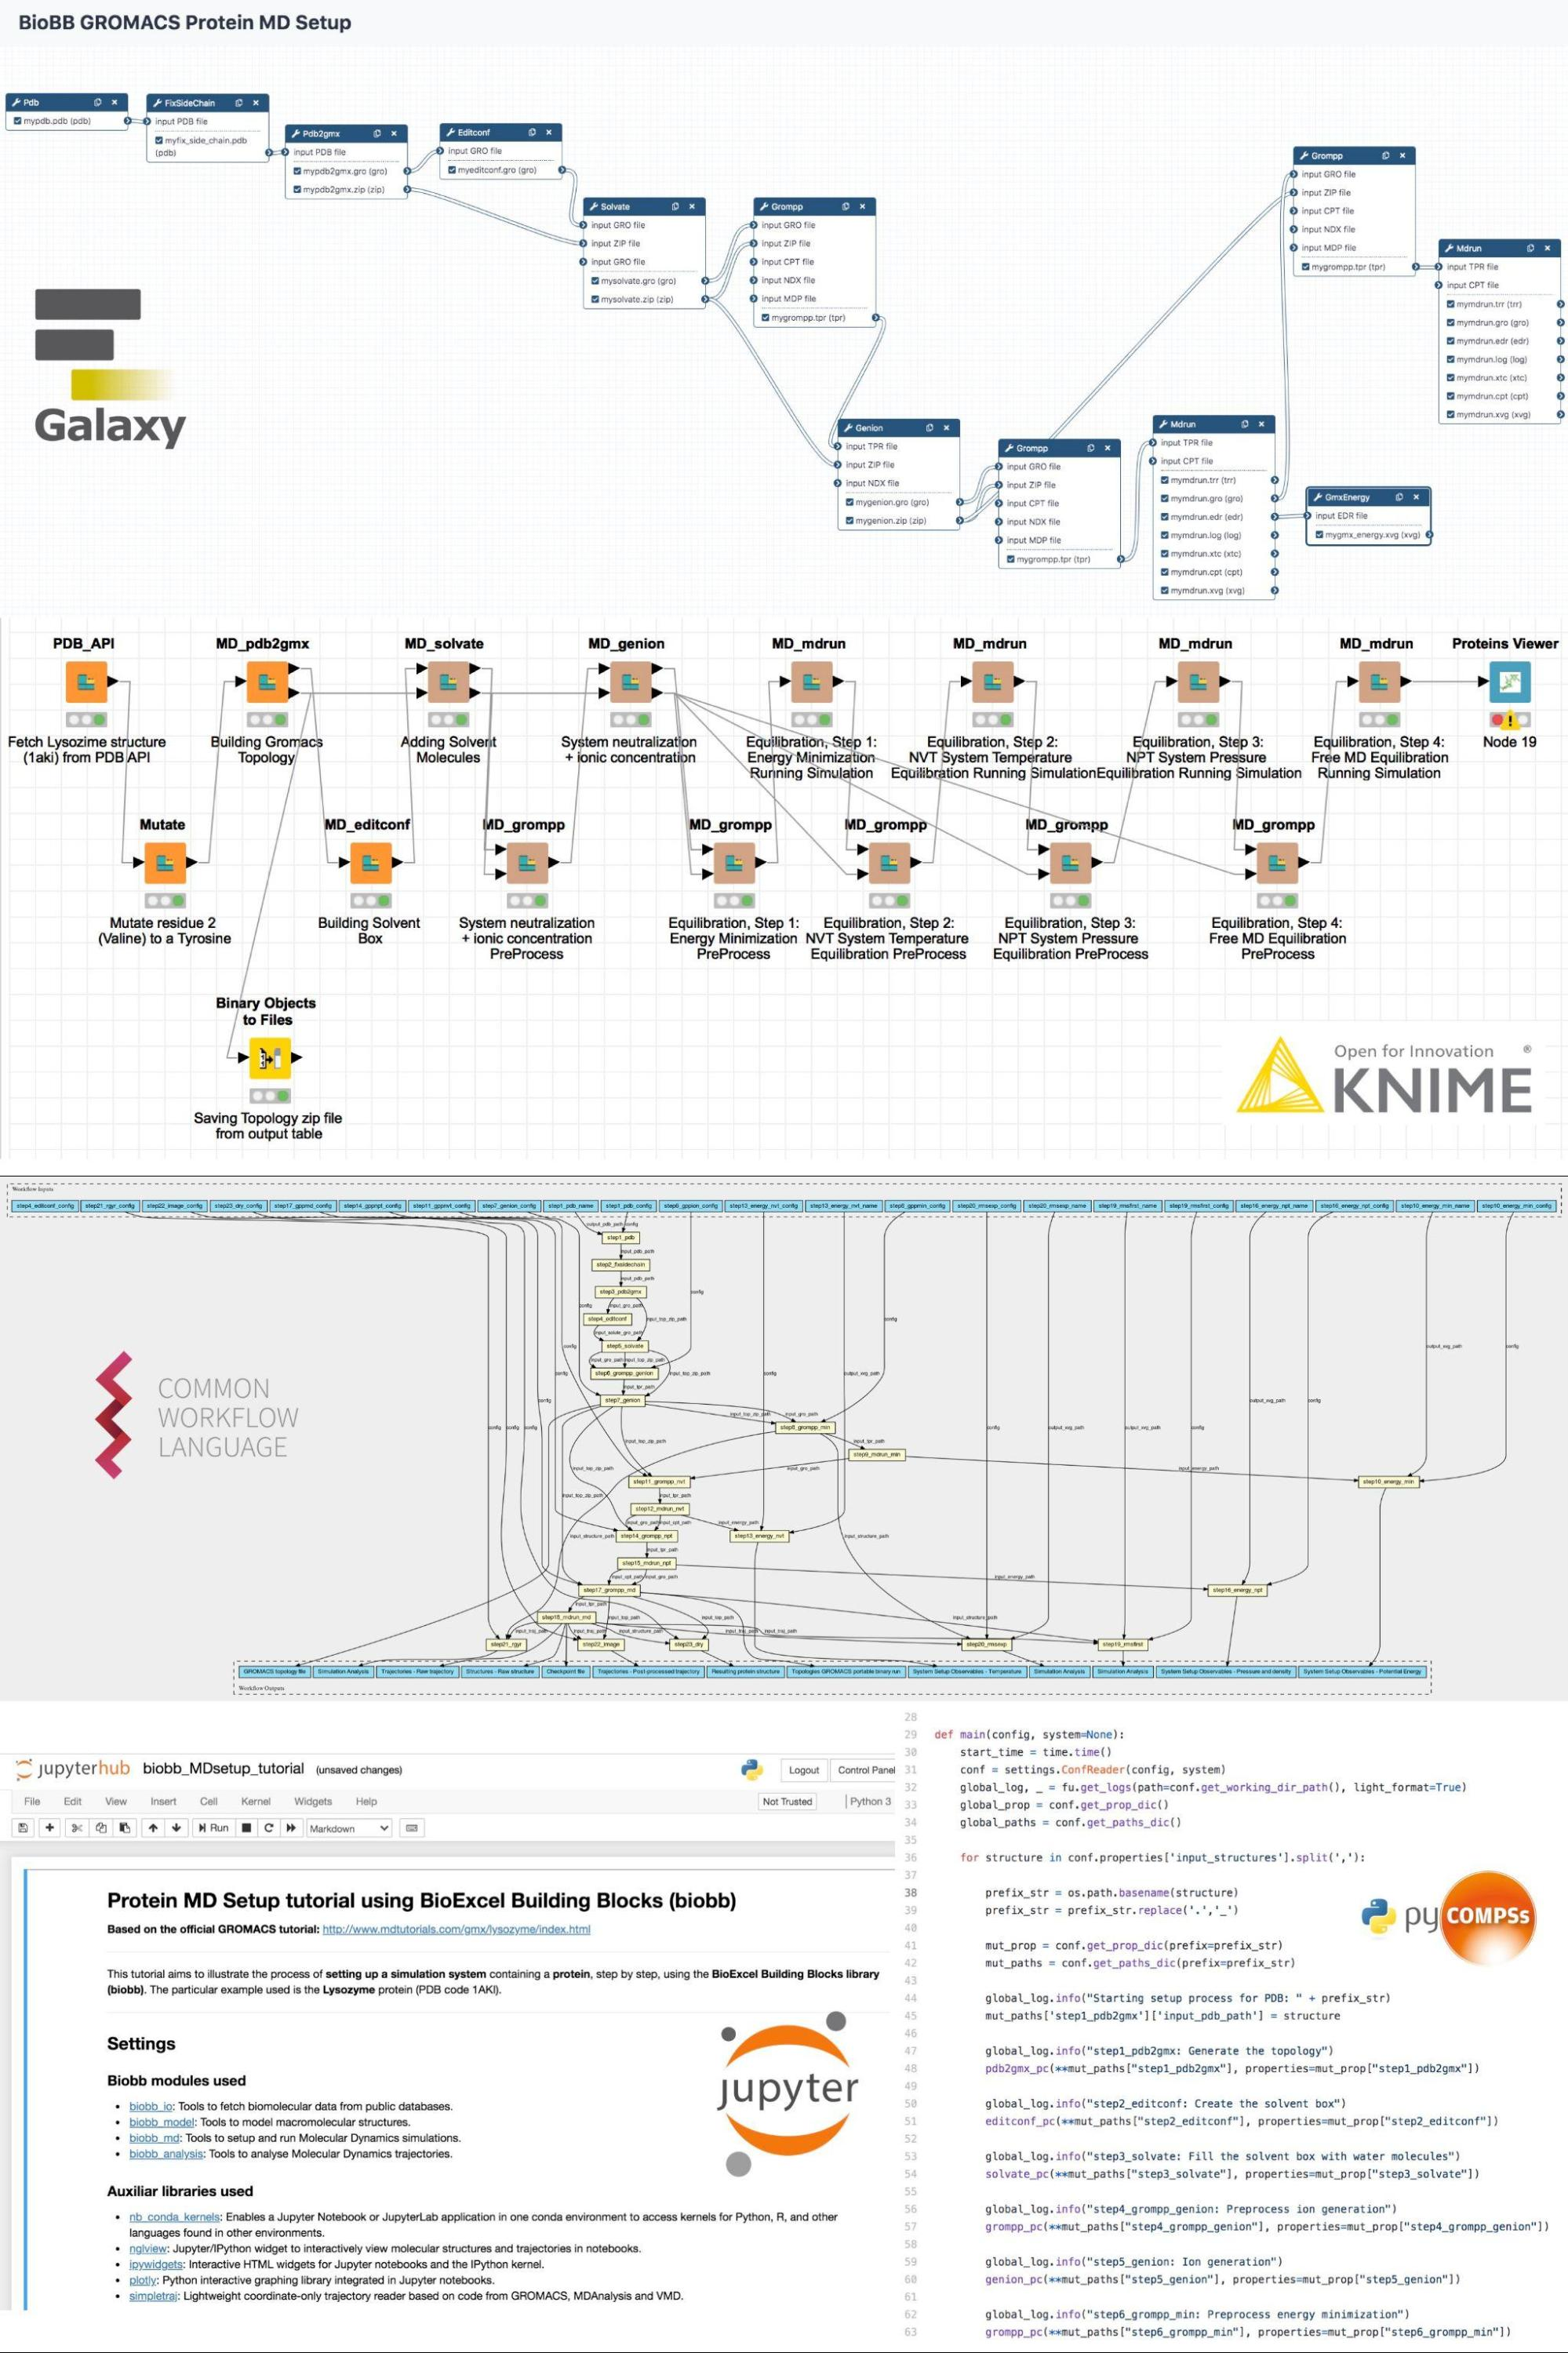
\includegraphics[height=19cm]{figures/ch06/figure2.png}
	\caption[Protein MD Setup transversal workflow]{\textbf{Protein MD Setup
  transversal workflow}. Assembled in with 5 different workflow
  managers using BioBB canonical building blocks. From top-left: Galaxy
  \cite{ch6-22}, KNIME \cite{ch6-23}, CWL \cite{ch6-24}, Jupyter Notebook \cite{ch6-25},
  PyCOMPSs \cite{ch6-26}.}
  \label{ch6:figure2}
\end{figure}

The transversal \footurl{https://workflowhub.eu/collections/3}{protein MD
setup workflow} was chosen as a real example that is readily
understandable by domain experts. More
\footurl{https://mmb.irbbarcelona.org/biobb/workflows}{complex pipelines}
involving a broader set of wrapped biomolecular tools have been
developed using the BioBB library, primarily as Jupyter Notebooks. A
selection of these have similarly been assembled for different WfMS
using the auto-generated bindings and uploaded to the
\footurl{https://workflowhub.eu/projects/11\#workflows}{WorkflowHub
repository}.

\subsection{Discussion}\label{ch6:discussion}

Early work on libraries of workflows fragments include Web Service-based
approaches where tools are wrapped and exposed using common,
interoperable data types in \footurl{http://biomoby.open-bio.org/}{BioMoby}
\cite{ch6-27} for bioinformatics and similarly
\footurl{https://en.wikipedia.org/wiki/CaBIG}{caBIG} \cite{ch6-28} for cancer
genomics. While these efforts were interoperable across WfMSs they
required a large up-front investment in agreeing to and adapting native
data to common RDF or XML representations.

The notion of \emph{abstract workflows} \cite{ch6-29}, structural workflow
descriptions separated from their concrete execution realisations and
augmented with Linked Data annotations, have been emphasised as
essential for reuse and consistency across workflow systems. Identifying
\emph{common motifs} for workflow operations \cite{ch6-30} (e.g.~Data
preparation, Format transformation, Filter, Combine) are important to
simplify and understand otherwise fine-grained workflow provenance
traces.

Most other efforts to standardise a set of disparate analytical tools
have been done within the scope of a single WfMS, allowing customised
user interaction, data visualisation, configuration and findability, for
instance
\footurl{http://www.taverna.org.uk/documentation/taverna-2-x/components/}{Taverna
components} had prototypical building blocks \cite{ch6-31} which were
instantiated at runtime by reference from a registry.
\footurl{https://docs.knime.com/2020-07/analytics_platform_components_guide/index.html}{KNIME
components and metanodes}, shared on the
\footurl{https://hub.knime.com/}{KNIME Hub} are frequently designed to be
interoperable, but with a perhaps weaker notion of component families.
The \footurl{https://toolshed.g2.bx.psu.edu/}{Galaxy toolshed} \cite{ch6-32} is
likewise populated with different sets of tool wrappers that are largely
made to be interoperable within a category.

The \emph{Common Workflow Language} (\textbf{CWL}) \cite{Crusoe 2022} has a strong
emphasis on interoperable command line tool descriptions, with
\footurl{https://www.commonwl.org/user_guide/07-containers/}{support for
containers} and Conda packaging, as well as
\footurl{https://www.commonwl.org/user_guide/17-metadata/}{support for FAIR
metadata} like contributors, license and EDAM ontology type annotations.
With multiple leading workflow engines now supporting CWL, and
experimental Galaxy support, this seems perhaps the most promising
candidate for both making and describing canonical workflow building
blocks, however we've identified a few stumbling blocks.

One obvious challenge is that the implementing WfMS needs to have CWL
support, along with support for either containers or Conda packaging to
find the described executables. While it is possible to run a CWL tool
directly using a \texttt{\#!/usr/bin/env\ cwl-runner}
\footurl{https://en.wikipedia.org/wiki/Shebang_(Unix)}{shebang} on POSIX
systems, this still requires pre-installation and possibly configuration
of a CWL engine like \footurl{https://pypi.org/project/cwltool/}{cwltool}
or \footurl{https://toil.readthedocs.io/en/latest/running/cwl.html}{Toil}
\cite{ch6-33}. However workflow engines have multiple dependencies and often
cannot easily be run from a container themselves\footnote{To execute the
  wrapped tool, a containerized workflow engine would need \emph{nested
  containers} which are not generally recommended for security reasons.
  It is possible to work around this limitation using
  \footurl{https://sylabs.io/singularity/}{Singularity} or
  \footurl{https://docs.bioexcel.eu/cwl-best-practice-guide/devpractice/containers/conda.html}{Conda}.}.

Within the CWL community it was originally envisioned that a wider set
of workflow systems would adopt CWL for tool description/execution, with
a subset implementing full CWL workflow support. This would allow shared
community effort for describing tools, say in the
\footurl{https://github.com/common-workflow-library/}{Common Workflow
Library}, rather than each WfMS needing to duplicate this tool wrapping
in separate repositories and languages. However, with the exception of
experimental tool support in Galaxy, in practice all CWL implementers
have gone for full workflow support.

Another challenge is that making a set of building blocks frequently
requires the use of \emph{shims}, for instance file conversion, small
search/replace operations or file renames. In a CWL approach these can
either be performed with an
\footurl{https://www.commonwl.org/v1.2/Workflow.html\#Expressions_(Optional)}{Expression}
using JavaScript snippets which only has limited access to file content,
or as an additional workflow step added before or after the main tool
step. This combination could then be nested as a subworkflow, similar to
KNIME's \emph{metanodes}, and would also be flexible by allowing
different containers or packages for any pre- or post-steps. Such a CWL
building block however becomes harder to access from a non-CWL WfMS,
because of lack of control over configuration/execution options for the
now nested CWL tools. In practice\footnote{It is worth mentioning that
  it would also be possible to generate WfMS-specific bindings from CWL
  descriptions (e.g.~as demonstrated with
  \footurl{https://github.com/common-workflow-lab/cwl2script}{cwl2script}
  for Bash,
  \footurl{https://github.com/common-workflow-lab/gxargparse}{gxargparse}
  for Galaxy,
  \footurl{https://github.com/common-workflow-lab/cwl2wdl}{cwl2wdl} for
  WDL), although this necessitates constraining the tool and workflow
  definitions to a limited mappable subset of CWL.}, executing a nested
CWL workflow from a native WfMS language would require the engine to
implement full CWL Workflow support (or delegate to a CWL engine).

For the main BioBB building blocks we implemented
\footurl{http://mmb.irbbarcelona.org/biobb/workflows}{demonstrator
workflows} that highlight how the tools should be used in different
workflow management systems; each having a primary exemplar using
Jupyter Notebook, which can be explored interactively using the
\footurl{https://hub-bioexcel-binder.tsi.ebi.ac.uk/h}{BioExcel Binder}. If
we consider the abstract demonstrator workflows as \emph{canonical
workflows} they are therefore very much active objects, but can also be
seen as \emph{workflow templates}, as any real use case will need to
specialise the workflow to tweak parameters, data selection etc.

We therefore also provide such workflow templates for multiple WfMS,
including CWL, PyCOMPSs and Galaxy. These are fairly disparate workflow
languages, yet by the use of the same canonical workflow building blocks
(which again invoke the same software binaries), such WfMS-specific
workflows effectively are instantiations of the same canonical workflow.

One challenge found is how to publish such canonical workflows in
registries like the \footurl{https://workflowhub.eu/}{WorkflowHub}. The hub
supports the registration of Digital Objects in the form of RO-Crate
\cite{Soiland-Reyes 2022}, with the option of abstract CWL for describing the canonical
workflow template, along with direct references to the workflow's GitHub
repository.

For instance in the RO-Crate for
\url{https://doi.org/10.48546/workflowhub.workflow.200.1} \cite{ch6-26},
which can also be
\footurl{https://rawcdn.githack.com/bioexcel/biobb_hpc_workflows/53958e7c278e53c277a7217057b785482f193f7f/ro-crate-preview.html}{rendered}
from GitHub, we have an entry for the
\emph{\footurl{https://rawcdn.githack.com/bioexcel/biobb_hpc_workflows/53958e7c278e53c277a7217057b785482f193f7f/ro-crate-preview.html\#workflows/MD/md_list.py}{main
workflow}} according to the
\footurl{https://w3id.org/workflowhub/workflow-ro-crate/1.0}{Workflow
RO-Crate profile}, detailing each canonical workflow building block used
(e.g.~\footurl{https://rawcdn.githack.com/bioexcel/biobb_hpc_workflows/53958e7c278e53c277a7217057b785482f193f7f/ro-crate-preview.html\#https\%3A//pypi.org/project/biobb-md/3.6.0/}{biobb-md
metadata}). Here the FAIR aspect of the building blocks to help software
citation is exercised, as the building block wrapper has one set of
authors, documentation and licence (Apache-2.0), while the wrapped
software
(e.g.~\footurl{https://rawcdn.githack.com/bioexcel/biobb_hpc_workflows/53958e7c278e53c277a7217057b785482f193f7f/ro-crate-preview.html\#https\%3A//doi.org/10.5281/zenodo.2564764}{GROMACS
metadata}) has different authors, licence (GPL-2.1+) and documentation.

However, the deposit of such RO-Crates in WorkflowHub results in one
registration entry per workflow language, which are not otherwise
related and may not even share the same source code repository. Thus,
we've identified the need for adding an overall \emph{canonical workflow
entry}, which can bring in workflow documentation and references shared
across WfMS implementations, including a set of links to the more
granular canonical workflow building blocks used by the workflow, but
also to the individual WfMS implementations as separate digital objects.

A similar question of granularity applies at the workflow tool level
\cite{ch6-4}, particularly for Findability and Accessibility, as we can
consider at lowest granularity the \emph{scientific method} in general
(e.g.~any algorithm for sequence alignment), followed by an
\emph{application suite} (bio.tools entry \cite{ch6-35}, homepage,
documentation), instantiated as a particular \emph{software
installation} (Debian package, Docker container) with its dependencies
at same level. The installation includes one or more \emph{software
executables} (a particular binary, a running service service), providing
at the highest detailed granularity level the specific types of
\emph{software functionality} (a particular mode of operation, choice of
analysis), for instance using certain command line flags.

For canonical workflow building blocks, with a focus on pluggable
composability, this is mainly defined at this high granularity level of
specific software functionality: explicit operations from an installed
tool, which are then combined in a workflow. This is indeed the level
WfMS tool definitions are typically done, e.g.~a CWL Command Line Tool
specifies a particular way to run a particular software binary. However,
to be an actionable CWBB, the building block needs to additionally
convey the lower granularity levels; particularly to support multiple
options for interoperable installation and execution, as well as
metadata at the most general level, such as documentation and scholarly
citations.

While workflow management systems typically only operate at the highest
granularity levels for execution details, and are frequently unaware of
(or not exposing metadata at) the more general levels, we argue that in
order for a Canonical Workflow \cite{cwfr} to follow and support FAIR
principles for itself and its data, the workflow management system need
to \emph{propagate structured metadata} about the tools used by the
workflow. We propose that in order to support the workflow's
applicability to multiple WfMS, the tools themselves must also have a
consistent packaging and formal description that enables consistent
computational invocation.

At the most general level, a canonical workflow built using such CWBBs
is even conceptually reproducible because the FAIR documentation of the
workflow, through its canonical workflow building blocks, identifies how
individual tools and software applications are composed, which in worst
case can be rebuilt using different installation methods in a different
WfMS, or in best case inspected to detect and cross-link the same
canonical workflow appearing in different WfMS instantiations. This view
of software as composition of other software typically also applies at
individual tool level, which themselves depend on programming language
runtimes, libraries, services and reference data.

\subsection{Requirements for Canonical Workflow Building
Blocks}\label{ch6:requirements-for-canonical-workflow-building-blocks}

Building on the experiences with BioBB, we here propose requirements and
recommendations for establishing Canonical Workflow Building Blocks
(CWBB) as implementations of \emph{canonical steps} introduced for
Canonical Workflow Frameworks for Research \cite{cwfr}.

The core purpose of a CWBB is to wrap a command line tool or other
software that can perform an operation as part of a computational
workflow. As such, the general advice for making software workflow-ready
applies \cite{ch6-37} (e.g.~easy to install, documented, parallelizable,
reproducible output), however a CWBB is also permitted to make use of
additional scripts or \emph{shims} to further adapt a third-party tool
for workflow use and for data interoperability across blocks.

The way tools are installed or invoked varies slightly across WfMS and
operating systems, therefore a CWBB should provide multiple methods for
distributing software; currently containers (Docker, Singularity) and
distribution-independent packaging (e.g.~Conda, Homebrew) are promising
by having reproducible install recipes and a wide range of open source
dependencies (e.g.~Java, Python). Additionally building blocks should
allow overriding execution paths, e.g.~for use with HPC module system
and hardware-optimised binaries.

The CWBBs should have sufficient annotations to be able to generate
bindings for different WfMSs and REST APIs, e.g.~parameter names and
descriptions, types and default values; enumerators for options, file
formats for inputs/outputs.

Building blocks should be grouped into families that are interoperable
through common data structures and file formats, as well as having joint
naming conventions for configuration options. A CWBB family should be
released as a single version following
\footurl{https://semver.org/spec/v2.0.0.html}{semantic versioning} rules,
which should have a corresponding persistent identifier (PID) \cite{McMurry 2017}.

Metadata for CWBBs should be captured following FAIR guidelines, and
distributed as part of the block family and resolvable from the PID as a
FAIR Digital Object. Metadata should include references to the CWBB
software distributions (e.g.~\footurl{https://quay.io/search}{quay.io}
container URL) as well as attributions, citations and documentation for
the wrapped tool.

Example workflows showing CWBB usage should be included in a
WfMS-neutral language such as Jupyter Notebooks, which may have
equivalent variants for each workflow binding. These workflows should be
registered in a workflow registry like WorkflowHub or Dockstore, and
assigned their own PIDs.

\subsection{Conclusions}\label{ch6:conclusions}

The proposed concept of Canonical Workflow Building Blocks can bridge
the gap between FAIR Computational Workflows, interoperable
reproducibility and for building canonical workflow descriptions to be
used and described FAIRly across WfMSs.

The realisation of CWBBs can be achieved in many ways, not necessarily
using the Python programming language together with RO-Crate as explored
here. In particular if the envisioned Canonical Workflow Frameworks for
Research become established in multiple WfMSs with the use of FAIR
Digital Objects, the different implementations will need to agree on
object types, software packaging and metadata formats in order to reuse
tools and provide interoperable reproducibility for canonical workflows.

Likewise, to build a meaningful collection of building blocks for a
given research domain, a directed collaborative effort is needed to
consistently wrap tools for a related set of WfMSs, chosen to target
particular use cases (a family of canonical workflows).

For individual users, a library of Canonical Workflow Building Blocks
simplifies many aspects of building pipelines, beyond the FAIR aspects
and data compatibility across blocks. For instance, they can benefit
from training of a CWBB family using Jupyter Notebooks, and then use
this knowledge to utilise the same building blocks in a scalable HPC
workflow with a CWL engine like Toil, knowing they will perform
consistently thanks to the use of containers.

While we have demonstrated CWBB in the biomedical domain, this approach
is generally applicable to a wide range of sciences that execute
pipelines of multiple file-based command line tools, however it may be
harder to achieve with more algebraic ``in memory'' types of
computational workflows, where steps could be challenging to
containerize and distinguish as separate block.

We admit that biomolecular research is quite a homogenous field with
respect to computational analyses and now becoming relatively mature in
terms of tool composability in workflows, building on the experiences of
the ``FAIR pioneers'' in the field of bioinformatics. Other fields, such
as social sciences or ecology, can have a wider variety of methods and
computational tools, often with human interactions, and may have to
adapt the software to be workflow-ready \cite{ch6-37} before using them as
Canonical Workflow Building Blocks. Domains adapting CWBB approach (or
workflow systems in general) should take note of the great benefits of
hosting collaborative events where developers meet each other and their
potential users, demonstrated in our field with events such WorkflowsRI
\cite{ch6-39} and Biohackathons \cite{ch6-40}.

The Common Workflow Language shows promise as a general canonical
workflow building blocks mechanism: gathering execution details of tools
along with their metadata and references, augmented with
\footurl{https://docs.bioexcel.eu/cwl-best-practice-guide/devpractice/partial.html\#using-abstract-operations-as-placeholders}{abstract
workflows} to represent canonical workflows. However, this would need
further work to implement our CWBB recommendations in full. Future work
for the Canonical Workflow Building Blocks concept includes formalising
and automating publication practises, to make individual blocks
available as FAIR Digital Objects on their own or as part of an
aggregate collection like RO-Crate.
